\section*{Problem  Set 1}

~\\
\begin{mdframed}
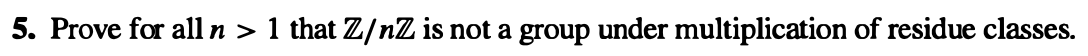
\includegraphics[width=400pt]{img/algebra--nf--1--problem-set-1-a4bb.png}
\end{mdframed}

{\it {\bf Intuition}: These are not groups because they all contain at least one element with no inverse.}

\begin{proof}
  Let $n > 1$ and let $X = \Z/n\Z$. Then $\bar{0} \in X$ and $\bar{1} \in X$, and $\bar{1}$ is a
  multiplicative identity for all elements of $X$. But $\bar{0} \times \bar{k} = \bar{0}$ for
  all $k = 0, 1, \ldots, n - 1$, therefore $\bar{0}$ has no inverse in $X$ under multiplication.
\end{proof}

~\\~\\
\begin{mdframed}
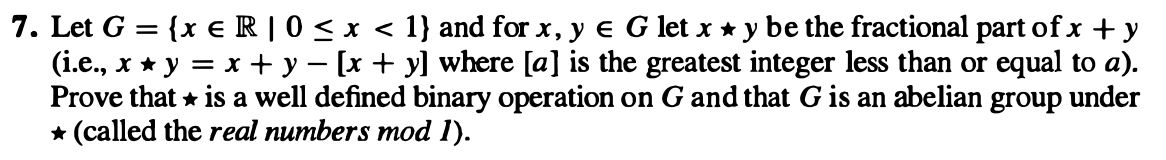
\includegraphics[width=400pt]{img/algebra--nf--1--problem-set-1-c770.png}
\end{mdframed}

\begin{proof}
  Let $r: \R \to [0, 1)$ be defined by $r(x) = x - \lfloor x \rfloor$. I.e., $r(x)$ is the fractional part of $x$.

  $\star$ is defined by $x \star y = r(x + y) \in [0, 1)$, therefore $\star$ is closed on $G = [0, 1]$.

  There is no ambiguity in the definition of its inputs, and it is defined by a deterministic
  procedure, and it is closed on $G$, therefore $\star$ is a well-defined binary operation on $G$.

  {\bf Existence of identity:}\\
  $0$ is an identity under $\star$ since $x \star 0 = r(x + 0) = r(x) = x$ for all $x \in [0, 1)$.

  {\bf Existence of inverses:}\\
  $0^\1 = 0$ since $0 \star 0 = r(0 + 0) = 0$.
  For $x \in (0, 1)$ we have $x^{-1} = 1 - x$, since $x \star (1 - x) = r(x + 1 - x) = r(1) = 0$.

  {\bf Associativity:}\\
  Let $x, y, z \in [0, 1)$. We have
  \begin{align*}
    x \star (y \star z)
    &= r(x + r(y + z)) \\
    &= r(x + y + z - \lfloor y + z \rfloor) &\text{definition of $r$}\\
    &= r(x + y + z)                         &\text{subtracting an integer doesn't affect fractional part}\\
  \end{align*}
  and
\begin{align*}
  (x \star y) \star z
  &= r(r(x + y) + z) \\
  &= r(x + y - \lfloor x + y \rfloor + z)    &\text{definition of $r$}\\
  &= r(x + y + z)                            &\text{subtracting an integer doesn't affect fractional part}\\
\end{align*}

Therefore $\star$ is associative.

  {\bf Commutativity:}\\
  $x \star y = r(x + y) = r(y + x) = y \star x$.
\end{proof}

\begin{remark*}
  Informally, the graph of $\star$ features a planar ``ramp​'' with height $0$ at $(0, 0)$ ending at
  a ``cliff​'' of height bounded above by $1$. The bottom of the cliff has height $0$ and lies along
  the line $y = 1 - x$; after the cliff it starts again from height 0 and increases again to a
  height bounded above by $1$. The point $(1, 1)$ is not in the domain.

  GPT4o produced this using numpy:
  \begin{mdframed}
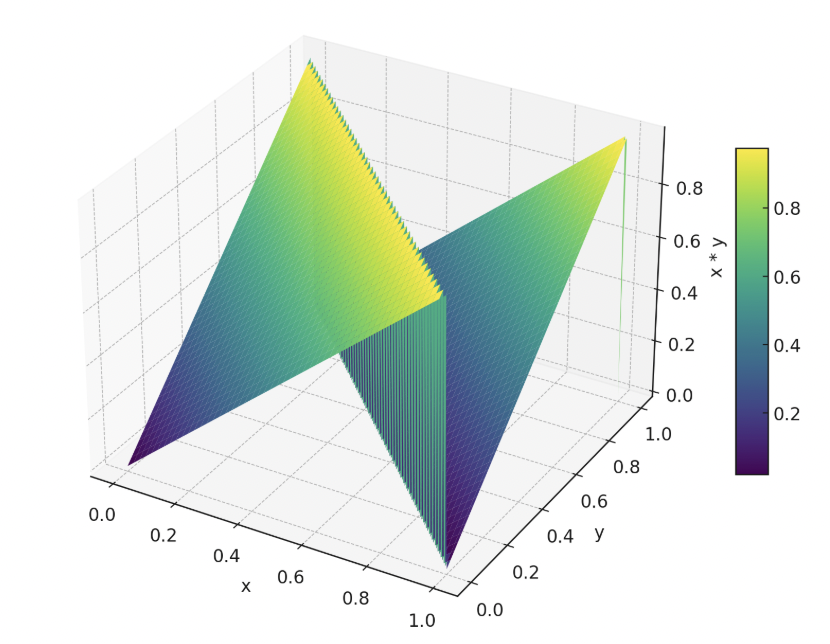
\includegraphics[width=300pt]{img/algebra--nf--1-6afd.png}
\end{mdframed}
  The fact that $0$ is an identity corresponds to the fact that the projection of the graph onto
  the $(X, Z)$ and $(Y, Z)$ planes yields the graph of $z = x$ and $z = y$ respectively.

  The fact that $1 - x$ is the inverse corresponds to the line of height $0$ along the $y = 1 - x$
  line in the $(X, Y)$ plane.
\end{remark*}




~\\~\\
\begin{mdframed}
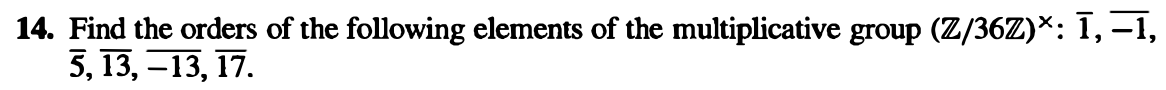
\includegraphics[width=400pt]{img/algebra--nf--1--problem-set-1-5539.png}
\end{mdframed}

\begin{proof}
  First note that the elements of $(\Z/36\Z)^\times$ are the residue classes given by integers that are
  coprime
  with
  $36$:
  $\{\bar{1}, \bar{5}, \bar{7}, \bar{11}, \bar{13}, \bar{17}, \bar{19}, \bar{23}, \bar{25}, \bar{29}, \bar{31}, \bar{35}\}$.
  (The residue class of an integer that shares a common factor with $36$ is not in the group
  because some power of that integer equals $0 \mod 36$ and $0$ has no multiplicative inverse.)

  There are $12$ elements, and we can compute the order of an element $x$ by doing calculations like
  % \begin{minted}{python3}
  % [(i, (x ** i) % 36) for i in range(1, 12+1)]
  % \end{minted}
  and observing when we first see a $1$.

  $|\bar{1}| = 1$ since $\bar{1}$ is the identity.

  $|\bar{-1}| = 2$ since $\bar{-1}^2 = (-1)(-1) = 1 \in \bar{1}$.

  Powers of $5$ (mod $36$) are $5, 25, 17, 13, 29, 1$ so $|\bar{5}| = 6$.

  Note that $13 = 5^4 \mod 36$. Therefore powers of $13$ (mod $36$) are $13, 5^8 = 25, 5^{12} = 1$
  so $\bar{13} = 3$.

  $|\bar{-13}| = |\bar{23}|$, and powers of $23$ (mod $36$) are $23, 25, 25, 13, 11, 1$ so $|\bar{-13}| = 6$.

  Powers of $17$ (mod $36$) are $17, 1$ so $|17| = 2$.
\end{proof}

\begin{remark*}
  As must be the case, we see that (a) the successive powers reduced mod $36$ only visit elements
  of the group, and (b) the orders we obtain ($1, 2, 3, 6$) are consistent with Lagrange's theorem.
\end{remark*}



~\\~\\
\begin{mdframed}
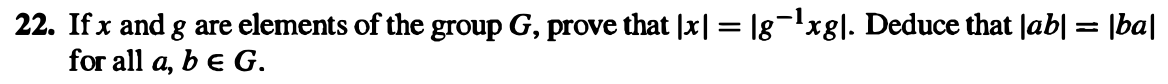
\includegraphics[width=400pt]{img/algebra--nf--1--problem-set-1-5058.png}
\end{mdframed}
\begin{proof}
  First note that for $k \in \N$ we have $(g^{-1}xg)^k = g^{-1}xgg^{-1}xg \cdots g^{-1}xg = g^{-1}x^kg$.

  Let $|x| = k$. Then $(g^{-1}xg)^k = g^{-1}eg = e$. Now suppose $(g^{-1}xg)^j = e$ for
  some $j < k$. Then we have $g^\1x^jg = e$. But multiplying on the left by $g$ and on the right
  by $g^\1$ yields $x^j = geg^\1 = e$, which contradicts $|x| = k$, therefore no such $j$ exists
  and we conclude that $|g^{-1}xg| = k$.


  Alternatively, suppose $x$ has infinite order. Then for all $k$ we have $x^k \neq e$,
  therefore $x^kg \neq g$ and $g^{-1}x^kg \neq e$. Therefore $g^{-1}xg$ is also of infinite order.


  Finally, we see from the result just proved that $|ab| = |a^\1(ab)a| = |ba|$ for all $a,b \in G$.
\end{proof}

\begin{remark*}
  The form of this conjugation operation reminds me of a change-of-basis procedure in linear
  algebra. It seems that here, like there, the conjugate result retains some properties of the
  original thing. Actually, more specifically, the result $(g^{-1}xg)^k = g^{-1}x^kg$ seems
  reminiscent of a diagonalization / eigenbasis change of basis procedure.
\end{remark*}


~\\~\\
\begin{mdframed}
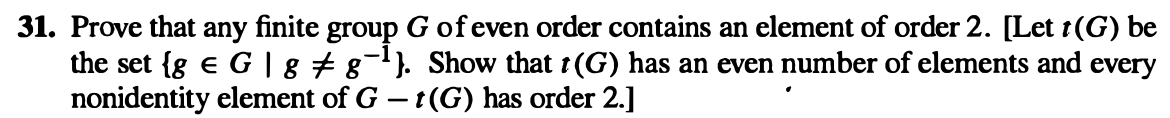
\includegraphics[width=400pt]{img/algebra--nf--1--problem-set-1-ca16.png}
\end{mdframed}

{\it {\bf Intuition}: the group can be partitioned into (A) the identity, (B) the non-identity elements
  that are their own inverse, and (C) those that are not their own inverse. |C| is even because
  they can be grouped into pairs. Therefore |A + C| is odd, hence B must be non-empty.}


We will use the following:

\begin{lemma}
  Let $X$ be a finite set. If there exists an injective mapping $f: X \to X$ that has no fixed
  points, then $|X|$ is even.
\end{lemma}

\begin{proof}
  Arrange the elements in some fixed order. Take the first element, say $a$, remove it from the
  set, and also remove $f(a)$ noting that this is a different element, and form the
  set $\{a, f(a)\}$. Continue until there are no more elements left. Note that it's impossible for
  there to be one left (Let such an element be $a$. Then $f(a)$ was also present. And yet $f(a)$
  was paired with no other element since $f$ is injective). Since we have partitioned $X$ into sets
  of size two, $|X|$ is even.
\end{proof}

Now we prove that every finite group $G$ of even order contains an element of order 2.

\begin{proof}
  Let $t(G) = \{g \in G | g \neq g^{-1}\}$ and consider $f: a \mapsto a^{-1}$. We see
  that $f: t(G) \to t(G)$ is a function since for $a \in t(G)$ we have
  $(a^{-1})^{-1} = a \neq a^{-1}$, therefore $a^{-1} \in t(G)$. Also, $f$ is an injection, since
  if $f(a) = f(b)$ then $a = f^2(a) = f^2(b) = b$. Finally $f(a) = a^{-1} \neq a$ by definition
  of $t(G)$, therefore $f$ has no fixed points. Since $f: t(G) \to t(G)$ is an injection with no
  fixed points, we conclude that $|t(G)|$ is even.

  Now consider the set $G - t(G) = \{g \in G | g = g^\1\}$. Since both $G$ and $t(G)$ are of even
  order, so is $G - t(G)$. But note that the identity $e$ is in $G - t(G)$ since $e^{-1} = e$,
  therefore there must also exist a non-identity element in $G - t(G)$. This element has order 2
  since for any such element $g$ we have $g^2 = gg^\1 = e$ and $g^1 \neq e$ since it's not the identity.
\end{proof}




~\\~\\
\begin{mdframed}
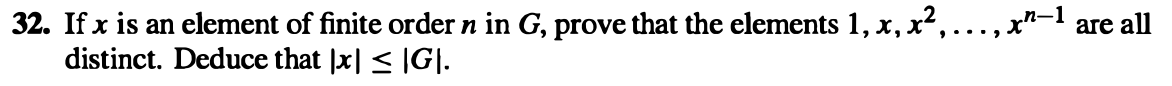
\includegraphics[width=400pt]{img/algebra--nf--1--problem-set-1-a008.png}
\end{mdframed}

\begin{proof}
  Let $G$ be a group and $x \in G$ with $|x| = n$. The claim is trivially true for $n = 1$. Suppose
  the claim is false for some $n > 1$. Then there exists $0 \leq i < j < n$ such that $x^i = x^j$.
  Therefore $x^{j - i} = e$ the identity. But this is a contradiction, since $|x| = n > j - i$.

  This implies that $|x| \leq |G|$ for all $x \in G$. To see this, suppose otherwise and let $G$ be of
  finite order $N$, and let $x \in G$ with $|x| = n > N$. Then we have $n$ distinct
  elements $1, x, \ldots, x^{n-1}$. But since $G$ is a group, it is closed under the operation, so
  these $n$ distinct elements are all elements of $G$, and we have a contradiction
  since $|G| = N < n$ by supposition. Alternatively, suppose $G$ is of infinite order.
  Then $|x| \leq |G|$ since $x$ is of finite order.
\end{proof}

% {\it {\bf Intuition}: It's true for the identity so let $x$ be a non-identity element. Then 1 and
%   $x$ are distinct. What about $x^2$? It can't be 1 since $x$ has order $n > 2$. And it can't be $x$ because $x$ isn't
%   the identity. So $1, x, x^2$ are distinct. What about $x^3$? It can't be 1 since $x$ has order $n > 3$. And it can't be $x$ because $x^2$
%   isn't the identity. And it can't be $x^2$ because $x$ isn't the identity. And so on.}



~\\~\\
\begin{mdframed}
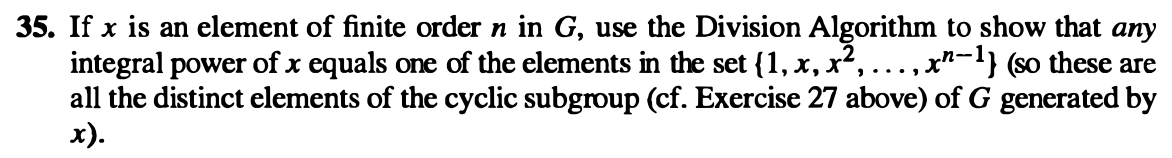
\includegraphics[width=400pt]{img/algebra--nf--1--problem-set-1-7561.png}
\end{mdframed}

\begin{proof}
  Let $x \in G$ be an element of finite order $n$. We wish to show
  that $x^a \in \{1, x, x^2, \ldots, x^{n-1}\}$ for all $i \in \Z$.

  By the Division Algorithm there exist unique $q, r$ such that $a = qn + r$ where $0 \leq r < n$.
  Therefore $x^a = x^{qn}x^r = (x^n)^qx^r = x^r \in \{1, x, x^2, \ldots, x^{n-1}\}$.
\end{proof}
